\chapter{The dataset}\label{cha:data}

This chapter introduces the dataset and prepossessing steps taken to enable information extraction and analysis of the provided data. In addition it introduces how the case analyzed in this thesis was found. 


% In the data set, there are three power plants that have pelton turbines with measurement of their needle position. More information about a pelton turbine can be found in chapter \ref{cha:data}. One of the power plants had recorded several issues with the control and behaviour of the needles during operation. There were many interesting events spread out over many of the power plants, but one major benefit with the pelton needle case, was that there was one plant with several reported issues for the same component. In most of the other cases, there were only recorded one incident on one plant, making them hard to analyze and validate. The fact that there also were two power plants in addition that had the same process signals without reported issues, opened up the possibility for testing and validating the chosen techniques not only on data from the faulty plant. This also introduced the possibility to validate how well and how easy the different techniques could adapt to new plants.    




% Based on the arguments above, the pelton needle case was chosen as the focus of the thesis. The following points were then defined as a basis for the analysis. 


\section{Dataset}\label{sec:dataset}
    Hymatek controls provided a third party dataset containing process information from $27$ hydro electric powerplants logged from $2013$ to mid $2017$. The data was not pre-prosessed in any way, and came just as it had been logged by the third party. A big part of the thesis has been spent on exploring the data, finding out what is logged and what can be used. The data was split into five folders, one for each year. In each folder several different files were stored. Table \ref{tab:data_files} shows the different file types that were found in the dataset. The file names indicated the frequency, sampling type and sampling duration of the data. The files were not separated by plants, only by date. Hence, a file containing data sampled every second for any given start and stop date, would contain all secondly sampled data from all plants for that given period. In addition to the datafiles, a meta-data file was provided where plant name and process signal for each tag could be found.    
    
    \begin{table}[]
        \centering
        \begin{tabular}{|c|c|c|c|c|}
            \hline
             Interval   & Average   & Max   & Min   & Actual    \\ \hline
             Daily      & x         & x     & x     & -         \\ \hline
             Hourly     & x         & x     & x     & -         \\ \hline
             Minutely   & x         & x     & x     & -         \\ \hline
             Secondly   & -         & -     & -     & x         \\ \hline
        \end{tabular}
        \label{tab:data_files}
        \caption{Table showing the available data for the different sampling frequencies}
    \end{table}
    
    The total size of all files exceeded $90$Gb, this meant that one could not simply just read all data into the ram and work with it from there. The information needed to be extracted for one plant at a time, for each of the different sampling rates, and stored in a way that enabled fast and efficient loading. All of the work with reading, processing and storing the data was done in python using the \textbf{Pandas} library. The \textbf{Pandas} package \cite{Mckinney2010} provides efficient and intuitive methods and data structures that serves as a great basis for data analysis. 
    
    
    
    \subsection{Old and new data format}\label{subsec:data_format}
        Regardless of sampling-rate and data type, the files were all on the same format. As seen in table \ref{tab:orig_data}, each line held a tag, a time of sampling and a process value. 
        
        \begin{table}[h]
            \centering
            \begin{tabular}{|c c c|}
                \hline
                 Tag        & Timestamp         & Value  \\
                 192390514  & 20170101000000000 & 0.897244155 \\
                 192391514  & 20170101000000000 & -0.549806237 \\
                 \hline
            \end{tabular}
            \caption{Example of the structure of the original datasets}
            \label{tab:orig_data}
        \end{table}
        
        Once a file was loaded the tag was replaced by the process-signal name found in the meta-data file. To enable interpretation and analysis of the data, it was decided that new datasets needed to be created. The format shown in table \ref{tab:plant_format} was chosen. When all samples from a given plant were extracted, and the tag replaced by the process name, the data matrix were reconstructed to hold the format shown in table \ref{tab:plant_format}
        
        \begin{table}[h]
            \centering
            \begin{tabular}{|c|c|c|c|c|}
                \hline
                Time stamp & P. variable 1     & P. variable 2    & ..    & P. variable n    \\ \hline
                time 1        & NaN         & $2$           & ..    & NaN         \\ \hline
                time 2        & $3.00$      & NaN           & ..    & $0.00214$\\ \hline
            \end{tabular}
            \caption{Example showing how the data could look in the data format for each plant after reconstruction is complete}
            \label{tab:plant_format}
        \end{table}

        
    \subsection{Overview of the datasets}
        Once the data was reconstructed as specified in subsection \ref{subsec:data_format} one could look into what information they held. The number of available process signals varied a lot, from above $250$ to below $20$, as can be seen in figure \ref{fig:process_signal_overview}. This was used as a first stage filtering to reduce the number of plants to examine. The plants with fewer than $30$ process-signals were dropped from the analysis, reducing the number of plants in the dataset to $15$.    
        
        \begin{figure}[h]
            \centering
            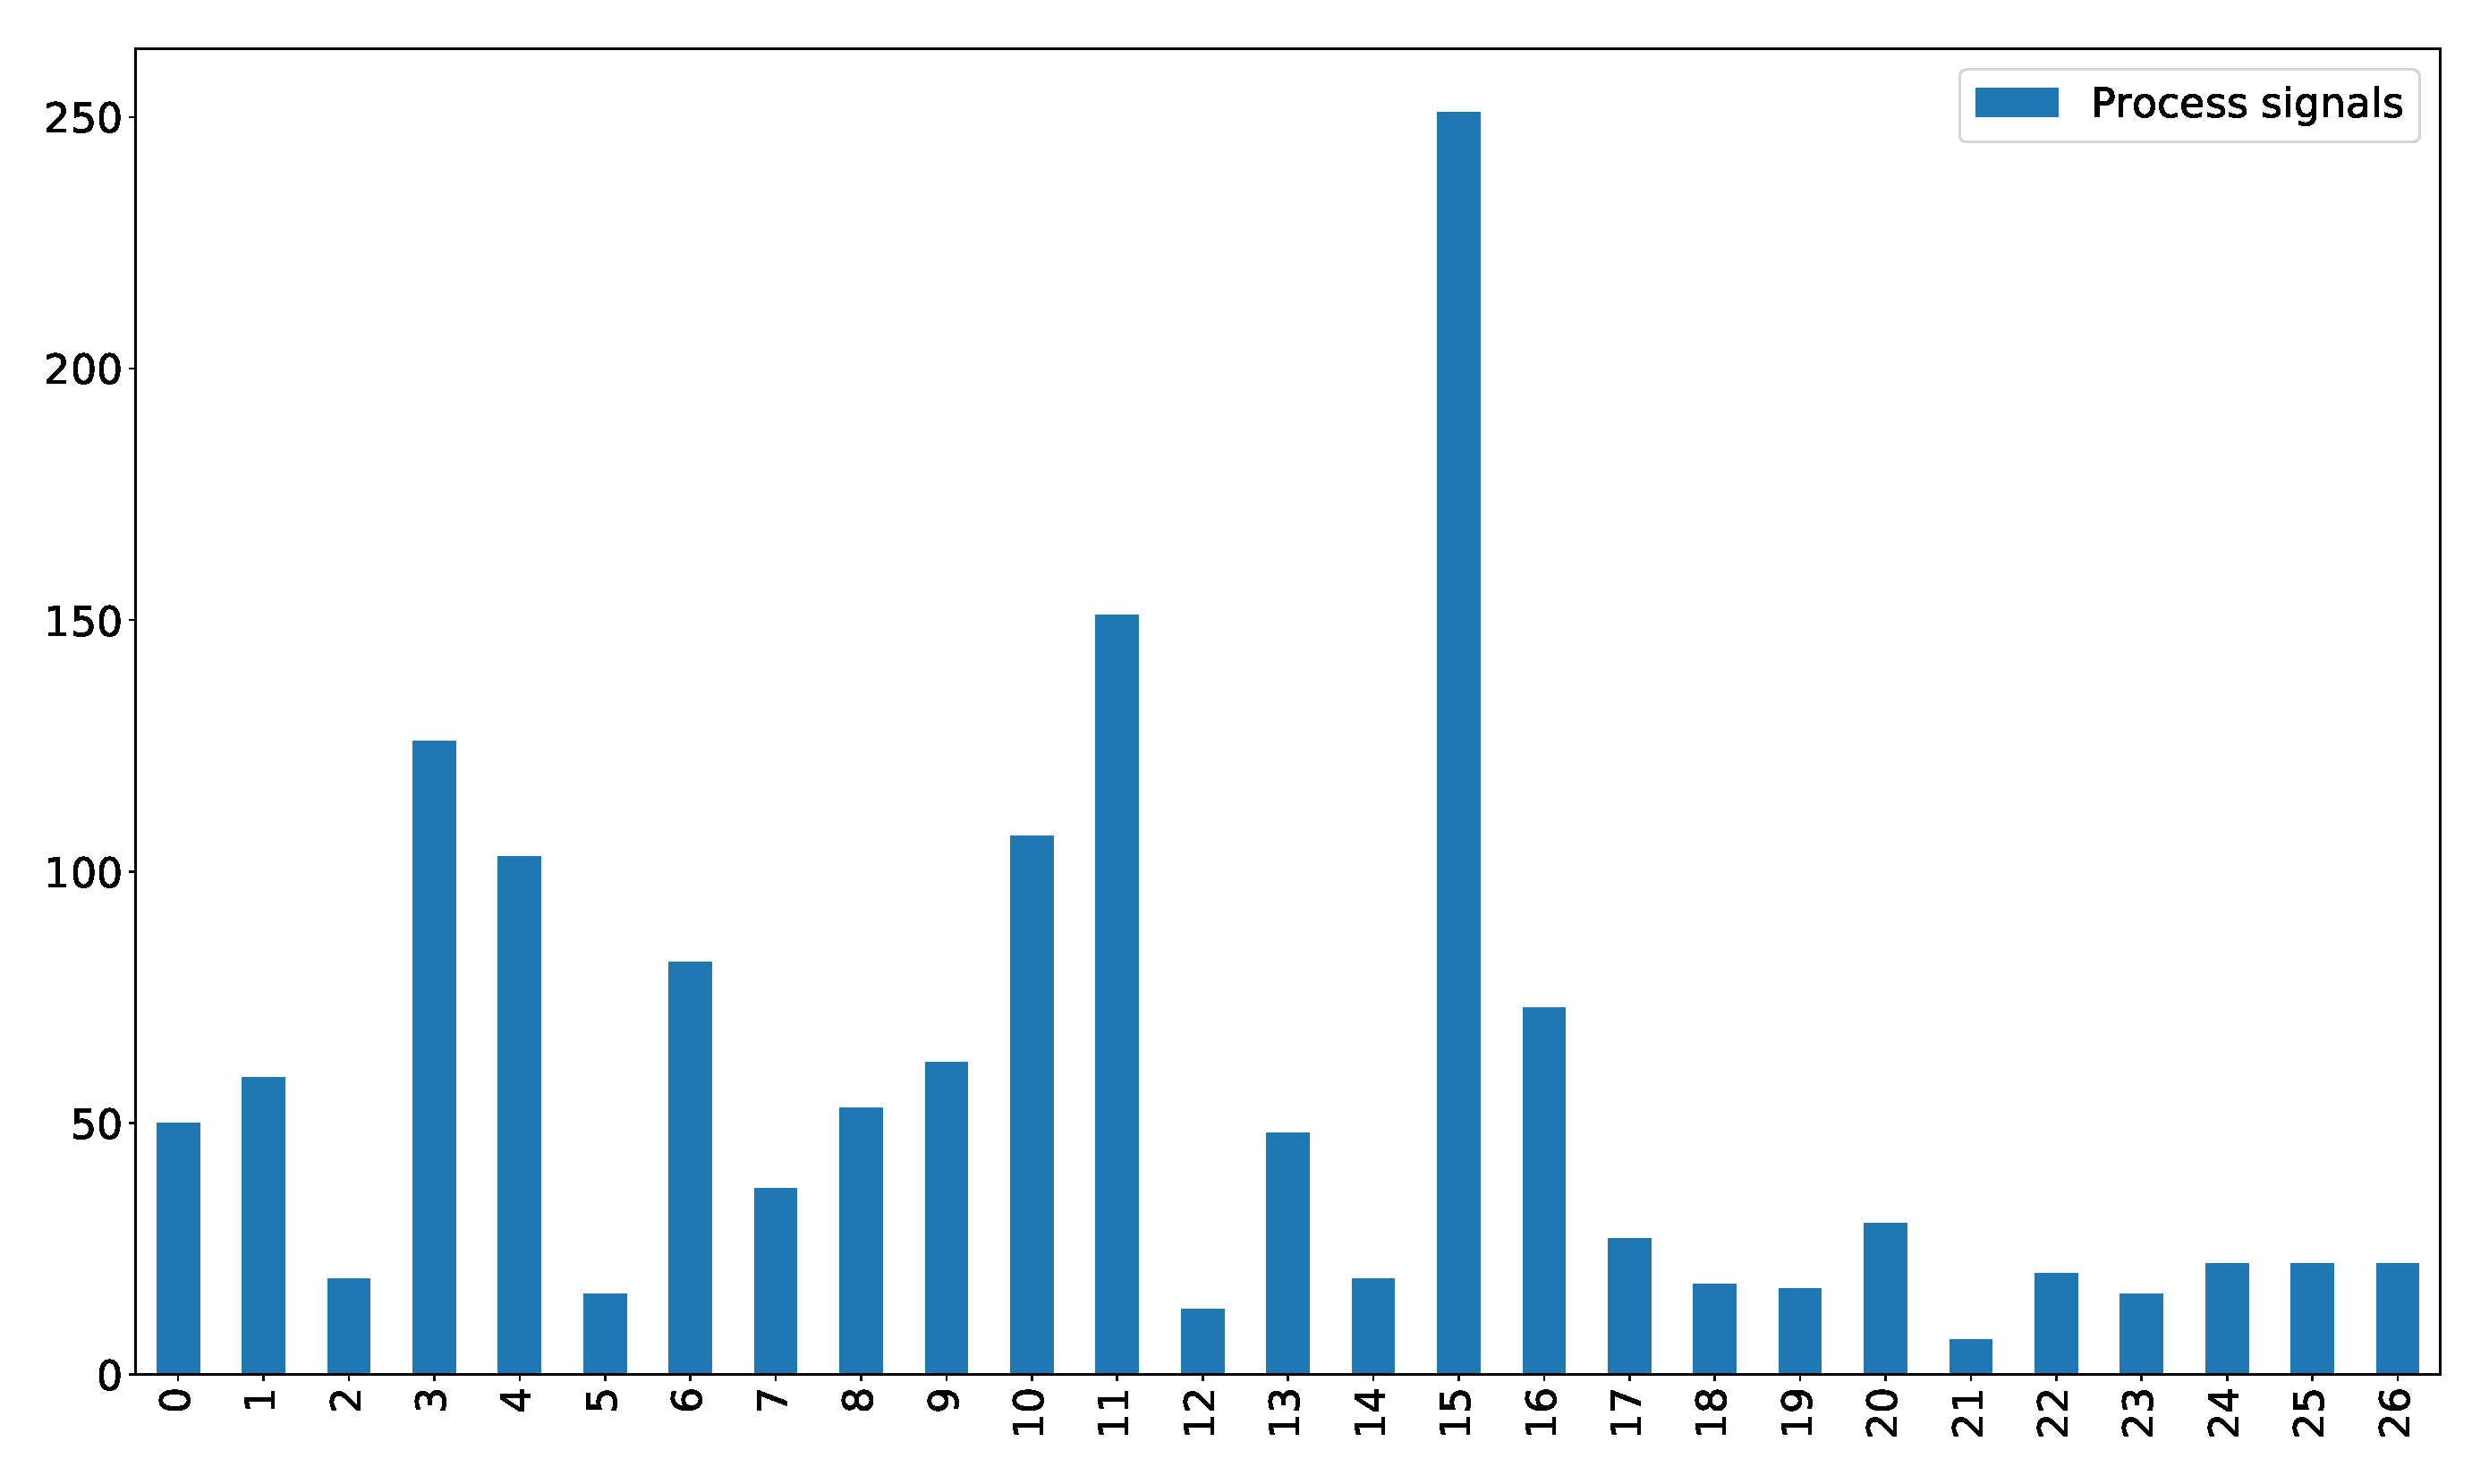
\includegraphics[width=\textwidth]{report/figures/data/plant_process_signals_overview.pdf}
            \caption{Overview of the number of process-signals for each of the 27 plants}
            \label{fig:process_signal_overview}
        \end{figure}
        
        After discarding the plants with few signals, the type of process-signals available were looked into. For a dataset to be useful, it is important that there is enough data and that there is data sampled from several parts of the plant. After all, the goal of the thesis is to find techniques that can help improve the knowledge about a plant beyond the scope of today's instrumentation, hence to find a link across different types of sensors and parts of the plant not known today is ultimately the goal. Figure \ref{fig:signal_type_overview} shows the different types of signals found in the different plant datasets. As can be seen temperature is one of the most common signals for all plants. There is also many signals of type "Def Type Måling", which is a common name that covers all signals not defined. Pressure, level, vibration, etc are signals covered by this tag. Since all of the remaining plants had process-variables of different types, none were removed. 
        
        \begin{figure}
            \centering
            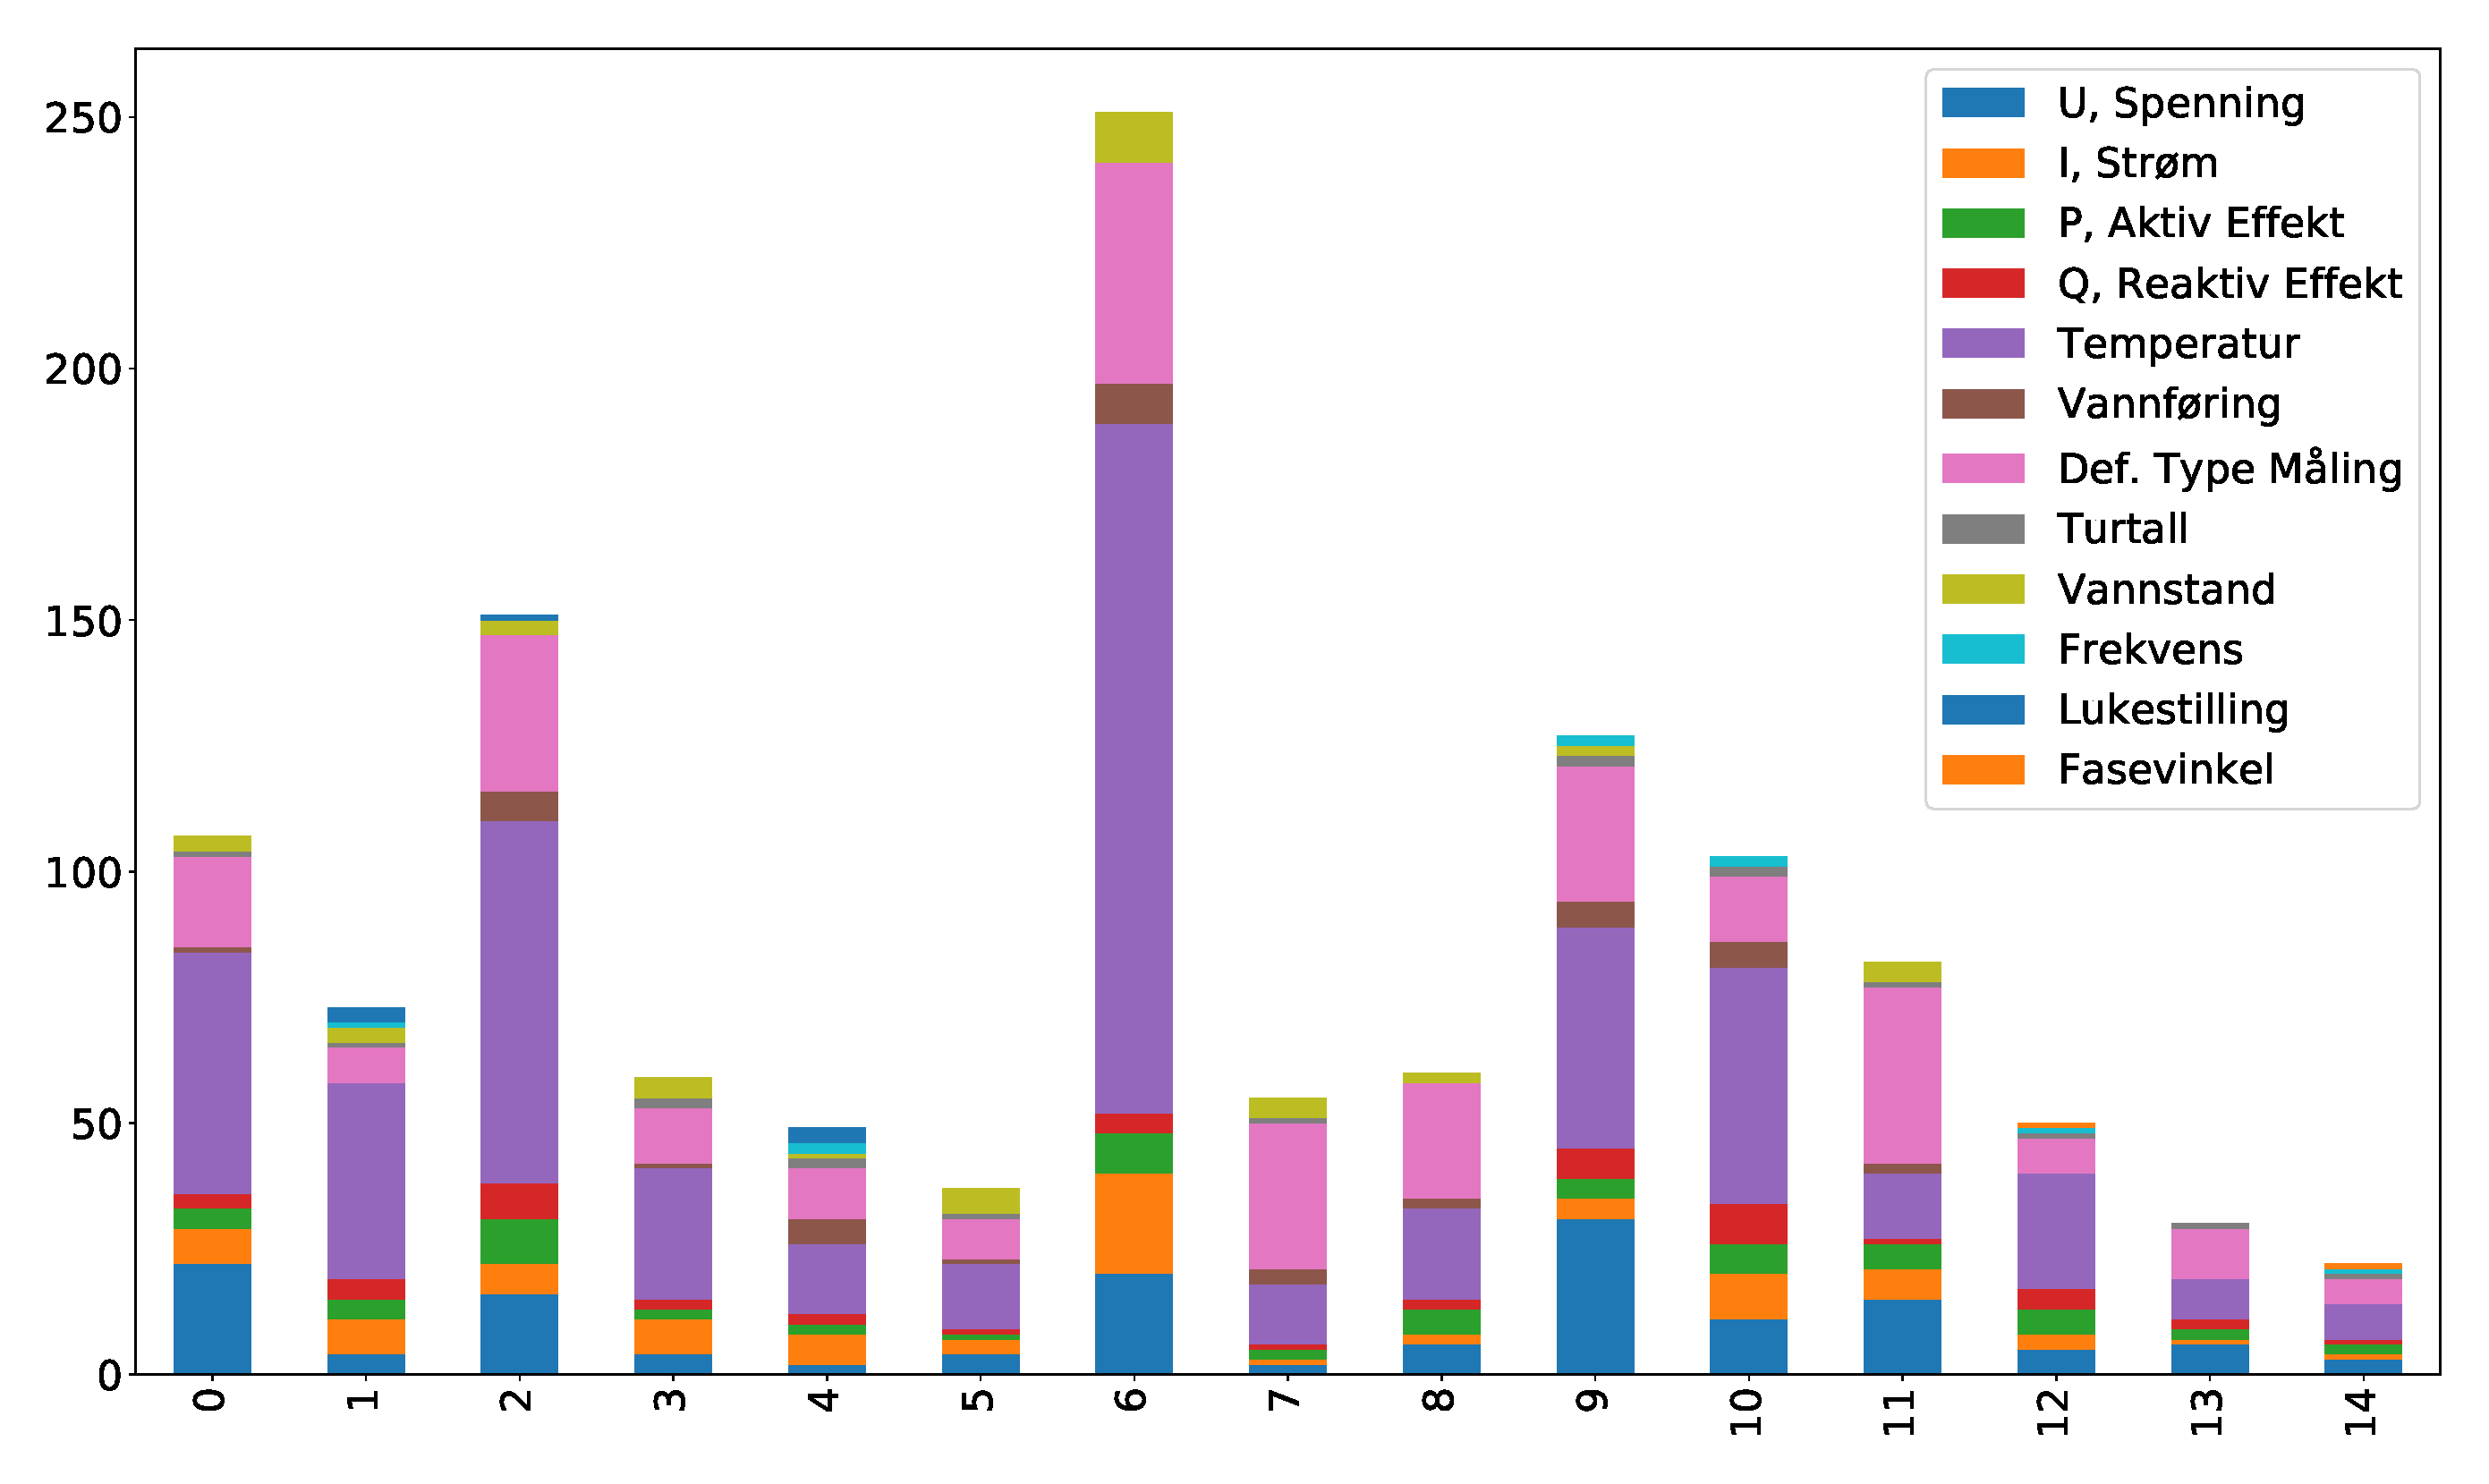
\includegraphics[width=\textwidth]{report/figures/data/plant_signal_types_overview.pdf}
            \caption{Figure showing the different variables found and the number of them in each plant dataset}
            \label{fig:signal_type_overview}
        \end{figure}
        
        It was decided to only use the datasets sampled every second. Using these datasets gave a snapshot of the plant state at a given time. Pandas has a lot of built in functionality that enables easy re-sampling, so that the average, max and min datasets could easily be recreated from this dataset if wanted.
        
        An issue arose when looking in detail at the plant datasets. Preferably, all process-signals should be sampled at the same time. This was however not the case, only at hourly resolution where the data matrices complete. At the frequency of seconds, there were many time-stamps were none of the process signals were sampled, and those that were sampled often only sampled one process-signal. This meant that one either had to work with only hourly sample rate, work with incomplete datasets or use some sort of interpolation technique to fill the gaps in the datasets. Why the third party has chosen to sample the data in such a way should be further investigated. Either the equipment used for sampling is not working as it should, or the varying sampling rate must be done on purpose. One can however, not find any reason for using such a sample scheme. This sheds light on the fact that having lots of data is not always a sign of quality. This issue will be further discussed in the analysis. Finally it was found that the data sampled in $2013$ had a very poor sample rate, and hence it was dropped from any further analysis. 
    % \subsection{Instrumentation}\label{subsec:instrumentation}
    %     what is there of instrumentation? refer to the data I have gotten         
        
    \subsection{The historical log of the plants }
        Once an overview of the data was created, the third party was contacted to see if they had any specific plant incidents that they wanted looked into. A historical log for all of the $15$ power plants were received, holding information about small to large incidents that had occurred during the sampling period. The level of details in the logged incidents were very varying from plant to plant. Some plants had reported over 200 incidents, while other barely exceeded 20. Many of the incidents were also minor incidents like a broken light bulb or non functioning tools. This made the work for finding interesting incidents time consuming. There were found several interesting incidents, but very few were reported to occur more than once. This is a a problem when working with machine learning and data analysis. Only having a limited number of faults can easily lead to overfitting. There is always a risk that the correlations and variable dependencies found can be caused by randomness. If one don't have enough erroneous observations to ensure that one is not modeling randomness and noise, the results can end up looking great, when in reality the solution is worthless on new data. 
        
        The third party reported an error with the needles of a Pelton turbine from one of the plants. As the power production decreases below $46\%$ one needle was reported to lag behind a needle it was operated with. This given plant has two Pelton turbines, with the same setup. These turbines have four needles each. When looking into the historical log of the plant, it was found that several more incidents with the Pelton needles were reported for the same turbine.
        
        A search through the $14$ remaining power plants, showed that there were two additional plants with Pelton turbines. One with four needles and one with five. These plants had however not reported any problems with the Pelton needles. This meant that one could assume to have data without error, which could be used as reference. This also meant that one could test the algorithms used on more plants, making sure one was not overfitting to one dataset. 
        
        
        
\section{Pelton needles case}\label{sub:pelton_needles}
    As mentioned, there was data available from three different power plants with Pelton turbines. As the incident reported that one needle was lagging behind another, it could mean that they were pairwise operated. To investigate how the needles were operated with regards to one another, scatterplots were created where each needle was plotted against the other. To enable this the needle process signals were pairwise extracted from the rest of the dataset, and all time-stamps where both needles were not sampled were removed. This meant that each time-stamp must be considered as a snapshot of the plant, and trends from one timestep to another not could be interpreted easily. The left figure in figure \ref{fig:pairwise_needles} shows an example of two needles that are pairwise operated. The opening of the needles are following each other linearly. The right figure show two needles that are not pairwise operated, at higher openings the needles seems to follow one another, but at lower openings this is not the case. This is because a Pelton turbine controls its power output by varying the number of active needles. Hence at full power all needles will be operated similarly, but at lower power some of the needles will not be operated. This is seen by all the samples found at zero opening for needle four, but at higher opening for needle three. 
    
    Further investigation showed that in addition to the plant that reported the incident, one of the other plants with Pelton turbines also had two turbines with pairwise operated needles. This meant that there were data available from four different turbines, that could be used for analysis. The third plant only had one Pelton turbine, and here the needles were not pairwise operated. The turbine used from 1 to 5 needles depending on the the produced power, and which needles were operated were rotated, most likely so that all needles should have the same amount of wear. Extracting periods where two or more needles are operated similarly could be used to extend the analysis.   
    

    \begin{figure}
        \begin{minipage}[b]{0.5\linewidth}
            \centering
            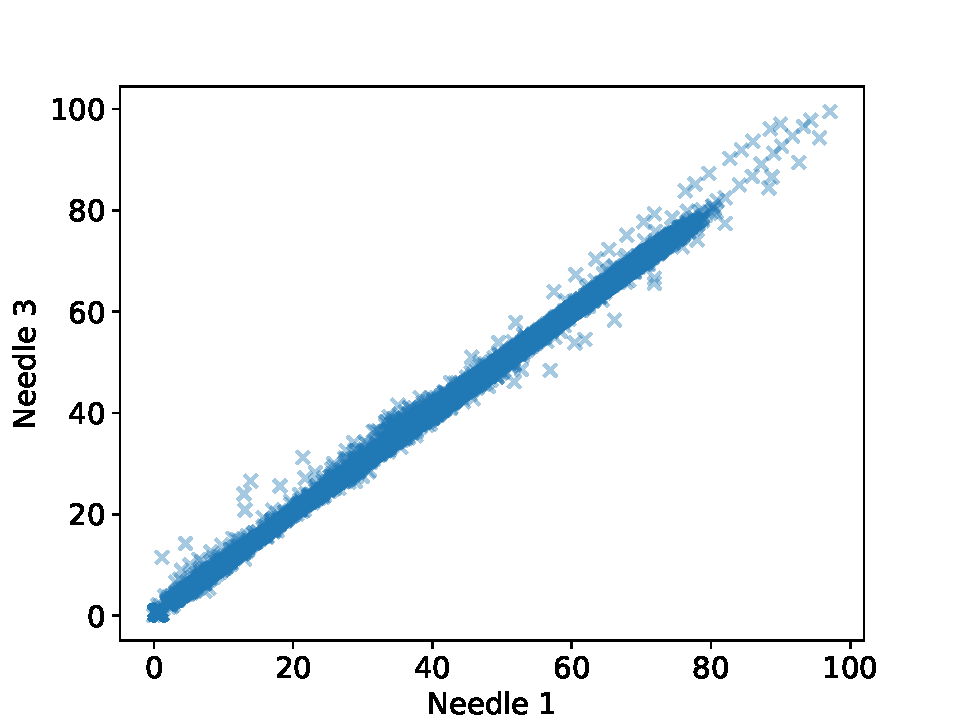
\includegraphics[width=\textwidth]{report/figures/data/Secondly samples needle [1,3] turbine 2 20170304:20170701.pdf}
            % \caption{Example of pair-wised operated needle openings, scatterplotted against each other}
            \label{fig:pairwise_neeldes}
        \end{minipage}
        \begin{minipage}[b]{0.5\linewidth}
            \centering
            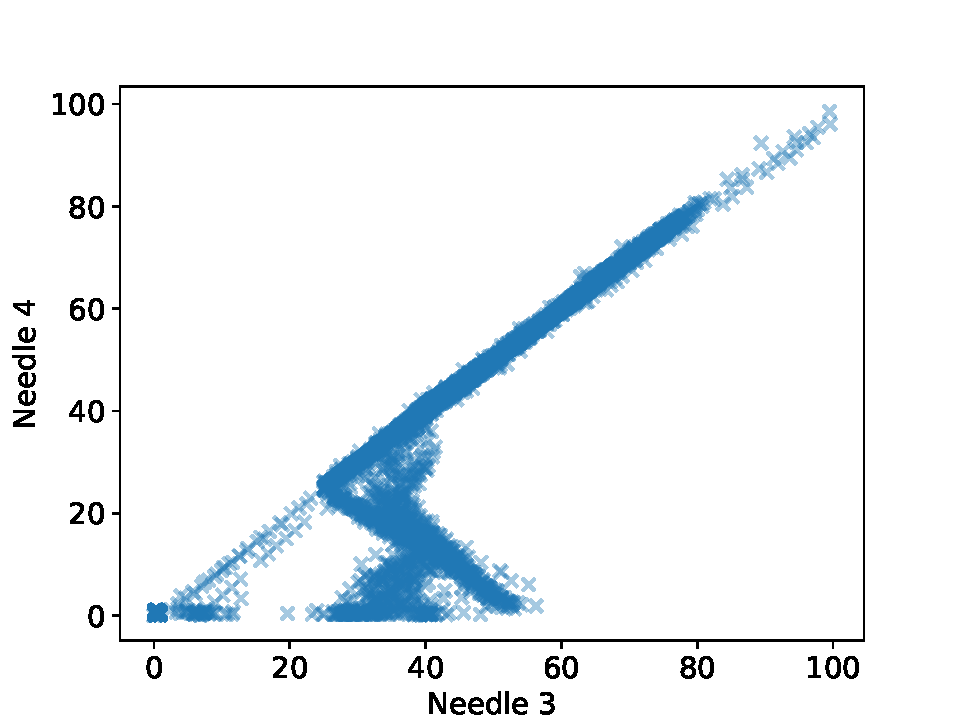
\includegraphics[width=\textwidth]{report/figures/data/Secondly samples needle [3,4] turbine 2 20170304:20170701.pdf}
            \label{fig:not_pairwise_needles}
        \end{minipage}
        \caption{Example of two needles openings scatterplotted against each other, in the left figure the needle pair is pair-wise operated, in the right figure they are not}
        \label{fig:pairwise_needles}
    \end{figure}
    
    
    Figure \ref{fig:plant1_needles} shows the scatterplot of the pairwise operated needlesfor plant 1. As can be seen, they all deviate from the pure linear pattern shown in figure \ref{fig:pairwise_neeldes}. The reported error occurred on turbine #$2$ with needle $4$ lagging behind needle #$2$. The plot in the bottom right corner clearly shows that there are several samples where the two needles are operating incorrectly. There is also tendencies to problems with needle #$1$ and needle #$3$ for the same turbine. Turbine $1$ is doing better, but for needle #$2$ and #$4$ there are some samples that are not as they should. 
    
    \begin{figure}
        \centering
        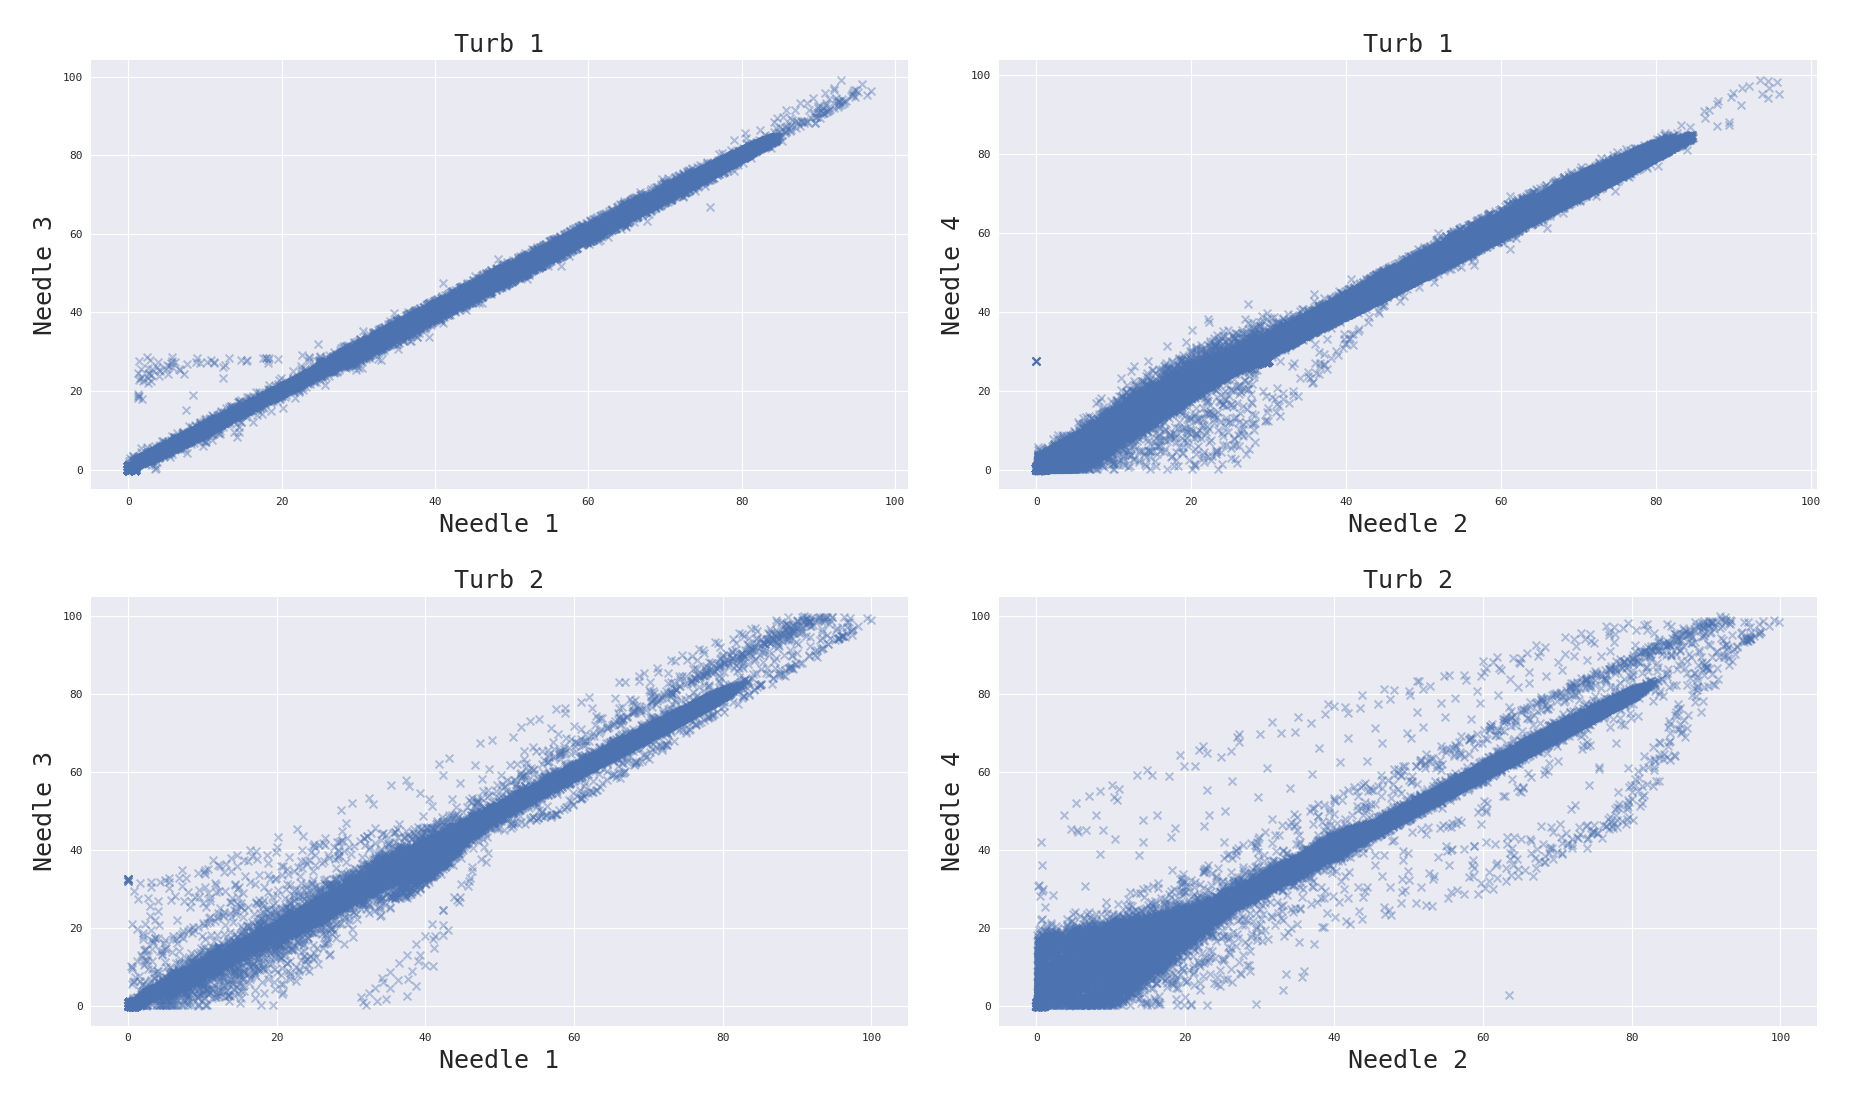
\includegraphics[width=\textwidth]{report/figures/data/plant1_needles.png}
        \caption{Pairwise operated needles for plant 1}
        \label{fig:plant1_needles}
    \end{figure}
    
    For plant #$2$ one can see in figure \ref{fig:plant2_needles} that turbine #$1$ has no sampling on needle #$1$, this means that this plant has three useful datasets. Based on plant 2 it becomes clear that there is something wrong with the needles for plant $1$. All needle pairs follow the linear pattern much better, and have very few outliers. This data can then be used for cheking if the algorithms wrongly detects outliers.
    
    \begin{figure}
        \centering
        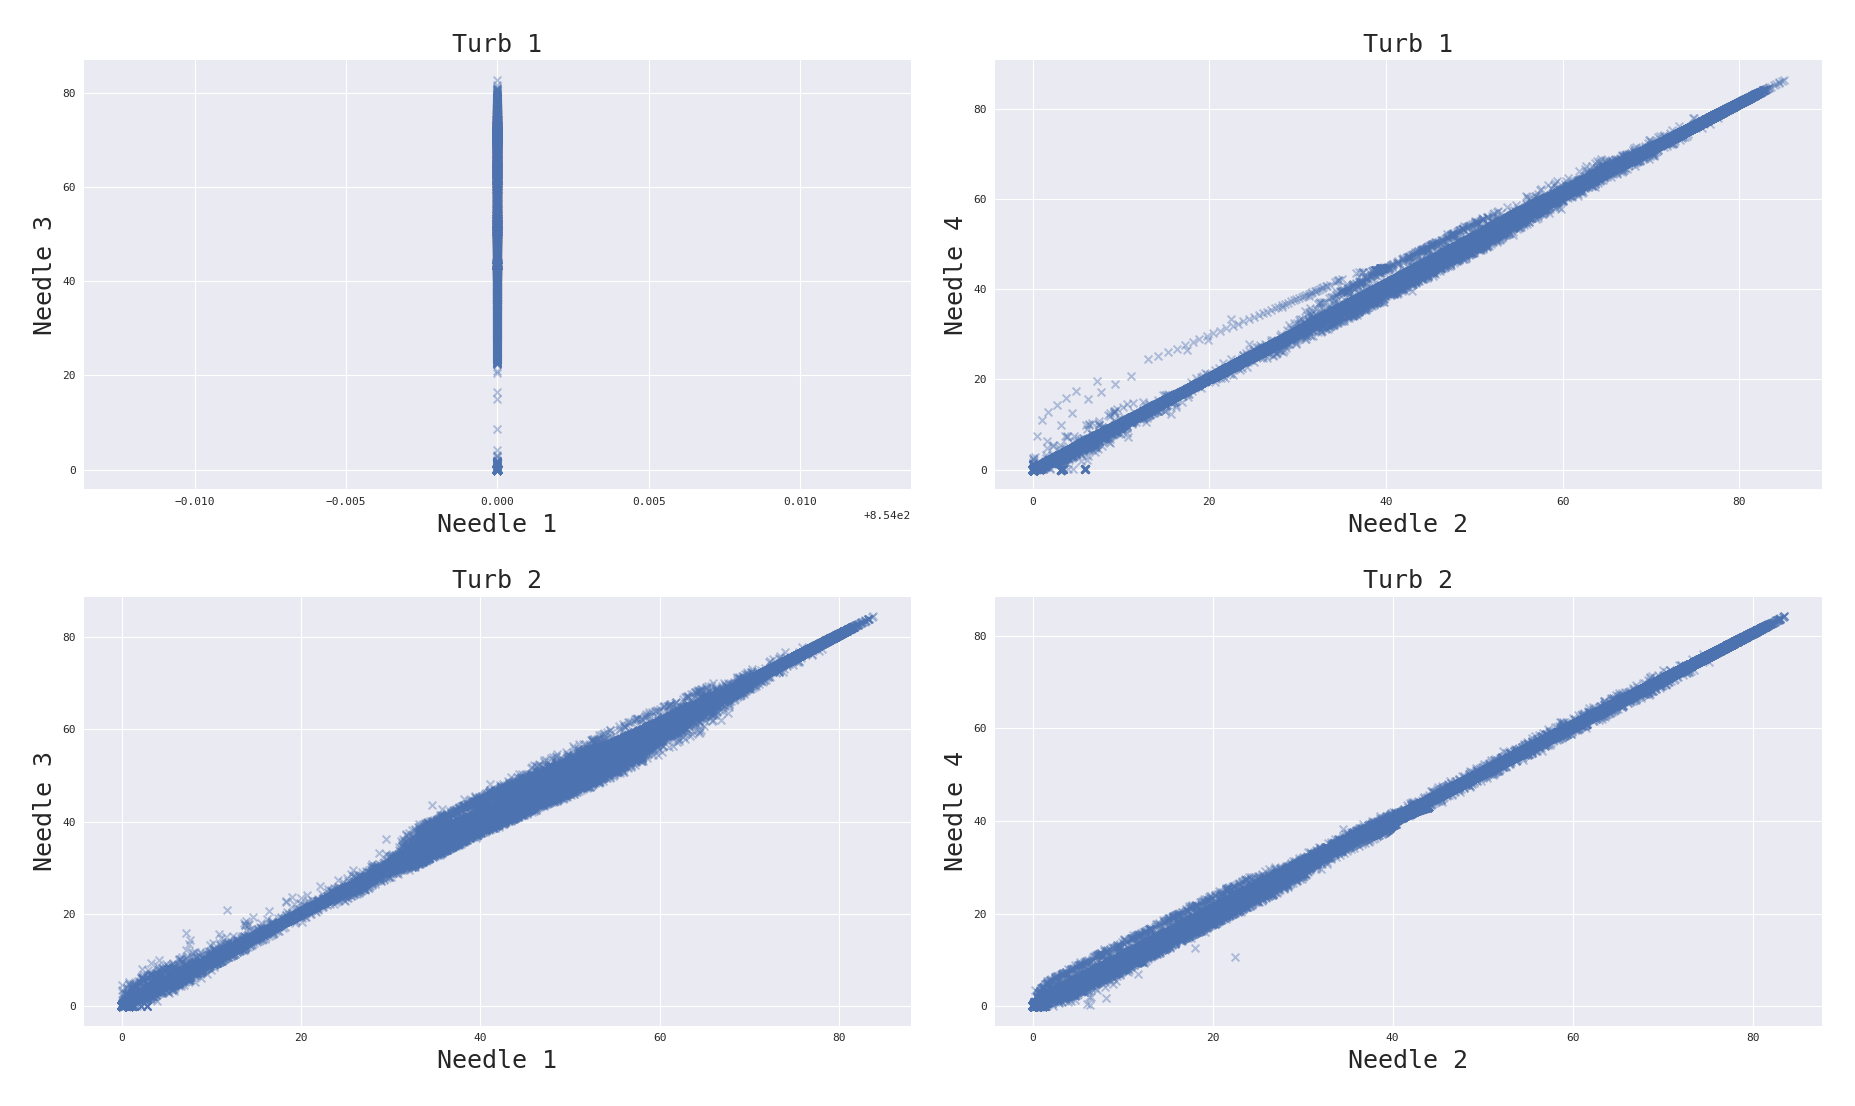
\includegraphics[width=\textwidth]{report/figures/data/plant_2_needle_plot.png}
        \caption{Pairwise operated needles for plant 2}
        \label{fig:plant2_needles}
    \end{figure}
    
    To further analyze if the Pelton needle case could be used, the needles position and the difference between them were plotted as seen i figure \ref{fig:plant1_needle_error}. The reported error from the third party occurred $03.03.2017$, in the plot one can clearly see that both the error and the RMSE between the two needles is much lower after the incident than before. It can also look like the error steadily grows from $01.10.2016$. Based on this the Pelton case was made the main foucs of the thesis. Looking into outlier detection, could one warn about the reported incident before it happend? Is it possible to trace the error to other process variables? This could improve the outlier detection, but also give valuable insight into what really happened. 
    
    \begin{figure}
        \centering
        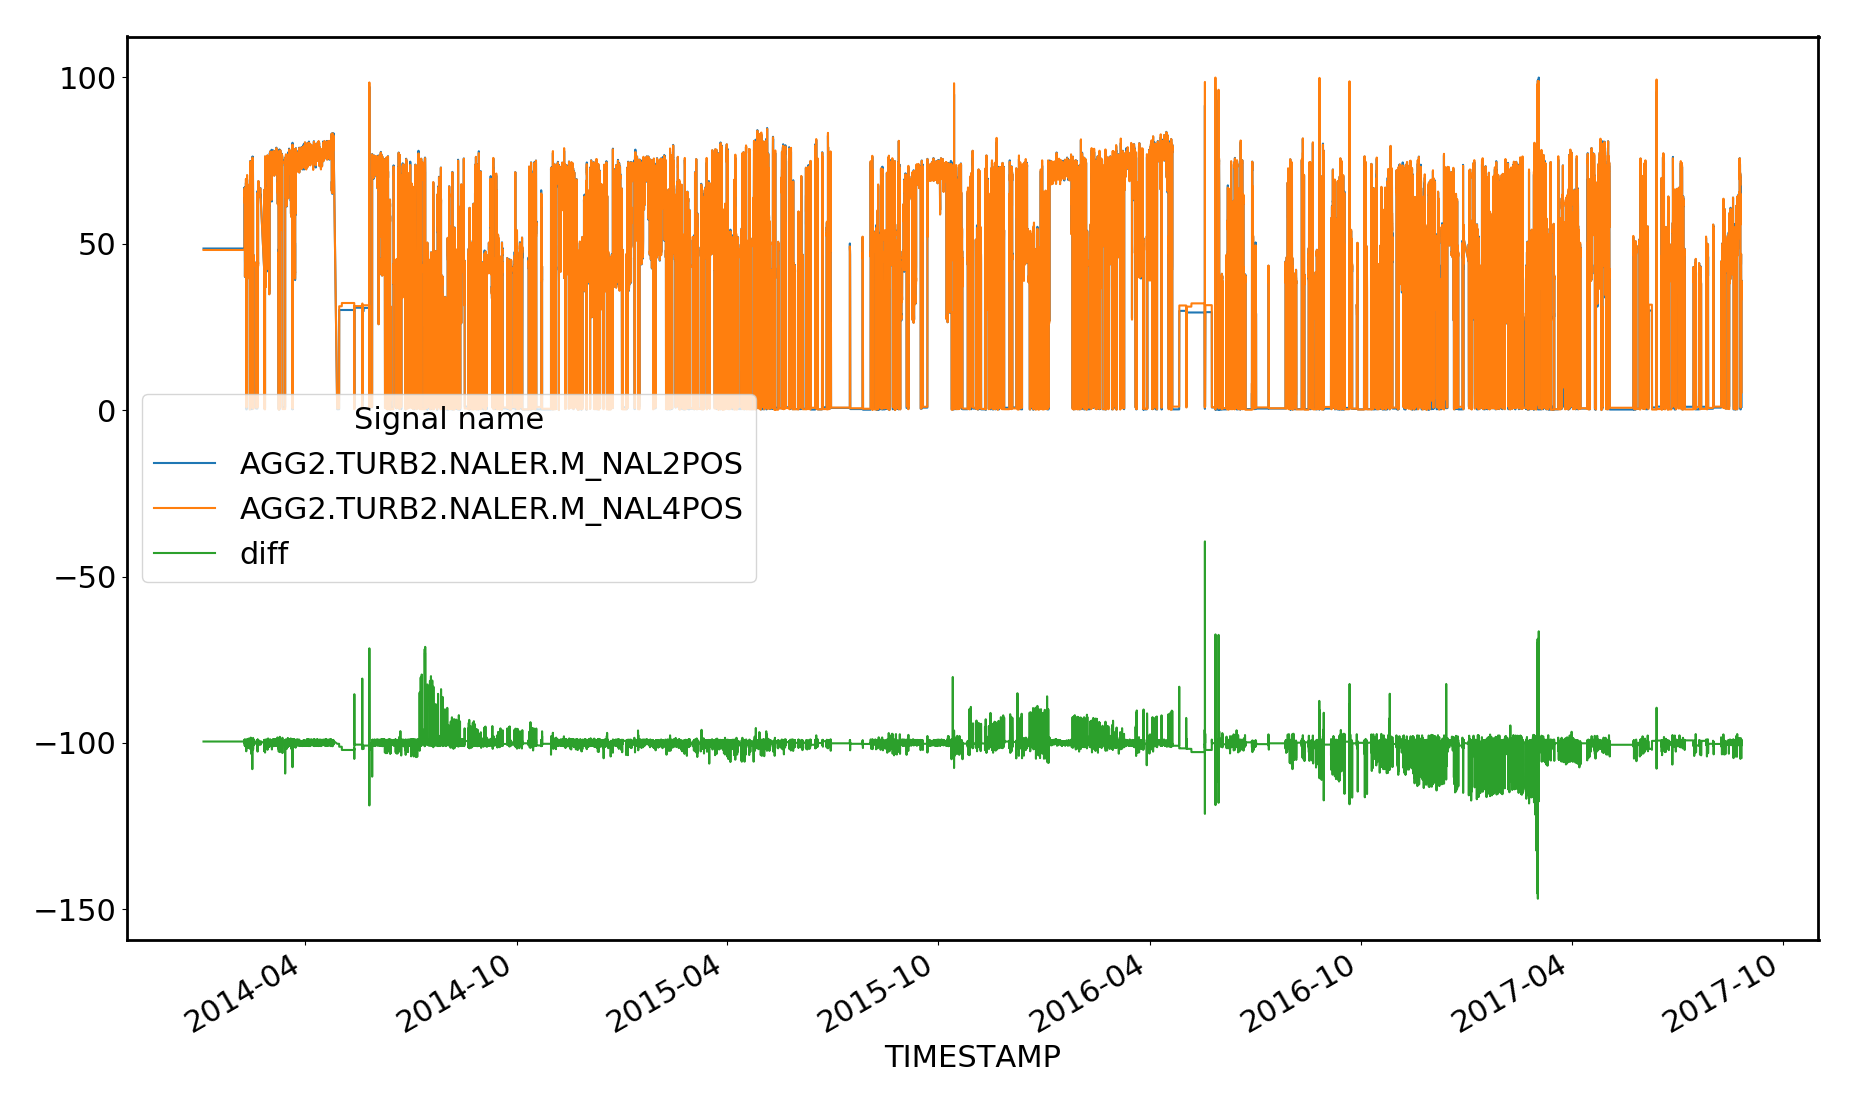
\includegraphics[width=\textwidth]{report/figures/data/turbine2_needle2_4.png}
        \caption{Overview of needle error for turbine 2, needle [2,4] on plan 1}
        \label{fig:plant1_needle_error}
    \end{figure}
    
    Finally, quality and available process variables varied a lot from plant to plant. One of the biggest issues was that the majority of the process signals were not sampled at a constant frequency. Often only one process-signal were logged for each time stamp giving a data matrix not straight forward to analyze. For the Pelton needle case, sample frequency and simultaneous sampling of several process signals were among the best in the dataset, making it a a good case study. 
    
% \section{Other process signals}
    

    
%     mention that this alone is a case one can build upon but to track the error to other processvariable would be very interesintg both for condition monitoring but also for identification of the fault and why it happened. 
    
    
%     It is important to understand that an outlier in the data does not necessarily mean that something is about to break. There is a possibility that the sample is an indication of a condition change in the equipmnet, but it might also be due to error in the measurement, noise or just a deviation in the ongoing process. This makes this kind of analysis even harder, an outlier might just be a coincident, that yields little to no information. 
    
     
     
    \subsection{Balanced datasets}
    
            Acquiring a balanced dataset, cite Tarassenko L. 
    
    "When building a dataset for training a data-driven model, it is important that data are acquired as uniformly as possible over the system’s entire operating range. A jet engine spends much of its time operating at “cruise” conditions, with much less time spent operating under takeoff or landing conditions. If training data were drawn randomly from the entire flight, then this would result in a strong bias toward cruise conditions, simply because there would be many more feature vectors derived from periods of cruise operation. A balanced dataset is constructed by rejecting feature vectors during steady-state conditions if the change in engine speed with respect to that associated with the previous feature vector is below a given threshold. The effect of this is shown in Figure 1, in which a histogram of feature vector speeds from the original dataset shows a very dominant peak in the range from 80 to $85\%$ of maximum shaft speed, corresponding to cruise conditions. After rejection of consecutive feature vectors with similar speeds, the distribution is much more uniform across the whole speed range. This type of approach is used"
    
    To acquire a balanced dataset all samples where the plant is not operable is removed. But I need to make sure I don't remove data where one needle is stuck but the other one is operated! Hence both need to be zero for me to remove the sample! 
    
    
    add figure or table showing the number of samples each day as the number of process variables are increased. 
    
    
    \subsection{Differencing}
    
    
    \subsection{Number of process variables included in the analysis}